\documentclass[xcolor=x11names]{beamer}

\usepackage[utf8]{inputenc}
\usepackage[T1]{fontenc}
\usepackage[english]{babel}

%------------------------------------------------------------

\usetheme{metropolis}
\usecolortheme{metropolis}

\definecolor{TaridesDarkBlue}{RGB}{10, 63, 92}
\definecolor{TaridesMidDarkBlue}{RGB}{1, 91, 140} %015B8C
\definecolor{TaridesMidBlue}{RGB}{3, 150, 216}   % 0396D8
\definecolor{TaridesBrightBlue}{RGB}{55, 180, 236} % 37B4EC
\definecolor{TaridesLightBlue}{RGB}{144, 216, 252} % 90D8FC

%------------------------------------------------------------

\usepackage{tikz}

\AtBeginSubsection[]
{
 \begin{frame}
  \vfill
  \centering
  %\begin{beamercolorbox}[sep=8pt,center,shadow=true,rounded=true]{title}
    \usebeamerfont{title}\insertsubsectionhead\par%
  %\end{beamercolorbox}
  \vfill
  \end{frame}}

\setbeamertemplate{blocks}[rounded][shadow=true]
\setbeamertemplate{itemize subitem}[bullet]

%------------------------------------------------------------

\usepackage{lmodern}

\usepackage{enumitem}

\usepackage{amsmath,amssymb,amsfonts}
\usepackage{stackrel}

\usepackage{xcolor}

\usepackage{listings,lstautogobble}

\usepackage{courier}

\usepackage{graphicx}

\usepackage{pifont}

\usepackage{hyperref}

\usepackage{changepage}

%?
\newcommand{\added}[1]{\textcolor{gray!60!cyan}{#1}}
% Subtitle
\newcommand{\subtt}[1]{\textcolor{gray!30!cyan}{#1}}

%------------------------------------------------------------

\lstset{language=caml,autogobble=true,
        commentstyle=\color{TaridesBrightBlue},
        basicstyle=\footnotesize\ttfamily,
        breaklines=true,
        morekeywords={val},
        morekeywords=[2]{int, string, file_perm, unit, dir_handle, file_descr, open_flag, bytes, bool, option, list, inet_addr, array, host_entry, socket_domain, socket_type, sockaddr},
        keywordstyle=[2]{\color{TaridesMidDarkBlue}}
        }
        
%------------------------------------------------------------

\usepackage{minted}

\DeclareUnicodeCharacter{3B3}{$\gamma$}
\DeclareUnicodeCharacter{3B9}{$\iota$}
\DeclareUnicodeCharacter{3A3}{$\Sigma$}
\DeclareUnicodeCharacter{2208}{$\in$}
\DeclareUnicodeCharacter{2200}{$\forall$}
\DeclareUnicodeCharacter{2203}{$\exists$}
\DeclareUnicodeCharacter{2217}{$\ast$}
\DeclareUnicodeCharacter{231C}{$\ulcorner$}
\DeclareUnicodeCharacter{231D}{$\urcorner$}
\DeclareUnicodeCharacter{21A6}{$\mapsto$}
\DeclareUnicodeCharacter{2082}{$_2$}

%------------------------------------------------------------

\usepackage{macros}

%------------------------------------------------------------

\title{\Saturn: a library of verified concurrent data structures for \OCaml~5}
\date{\today}
\author{
  Clément Allain (INRIA Paris) \\
  Vesa Karvonen (Tarides) \\
  Carine Morel (Tarides)
}

\begin{document}

\maketitle



\begin{frame}{Plan}
  
 \begin{itemize}[label=\ding{114}]
     \item Why \Saturn ?
     \item What is in \Saturn ?
     \item Optimizations and benchmarks
     \item Testing
     \item Verification
 \end{itemize}   
 
\end{frame}

\begin{frame}{Why \Saturn ?}
    \hfill\small{\href{https://github.com/ocaml-multicore/saturn}{Github: ocaml-multicore/saturn}
\vfill
    \begin{itemize}[label=$\bullet$]
        \item A collection of concurrent-safe data structures for \OCaml~5: 
        \begin{itemize}[label=$\diamond$]
            \item well-tested
            \item benchmarked
            \item optimized
            \item verified
        \end{itemize}
        \item<2-> Writting concurrent code is hard 
    \end{itemize}
    }
    \vfill
\end{frame}

% Pour faire plus simple:
% - Saturn = lib de structure de donnée parce que :
%   + c'est déjà diff en séquentiel
%   + et ça le devient encore plus concurrent (c'est l'enfer)
%   -> tu veux pas le réécrire toi meme et c'est donc important d'avoir une bonne lib de structure de données concurrente


% En fait meme les structures de données les plus simples en séquentiel comme une queue c'est pas facile en concurrent. D'ailleurs, j'ai cherché sur git hub en cherchant Atomic dans le code ocaml sur github (que j'ai anomysé)

% Expliquer Atomic -> ça c'est un morceau de code ocaml qui utilise les primitives 

%En concurrence tout devient complexe meme une queue, donc les gens le font eux-meme et c'est pas une bonne idée
\begin{frame}[fragile]{Buggy queue with size}     
    \begin{lstlisting}
        module Queue = Saturn.Queue 
        type 'a t = {size : int Atomic.t; queue : 'a Queue.t}

        let create () = 
            {size = Atomic.make 0; queue = Queue.create ()}
        
        let push t msg =
          Atomic.incr t.size;
          Queue.push t.queue msg
        
        let pop_opt t =
          match Queue.pop_opt t.queue with
          | Some elt ->  Atomic.decr t.size; Some elt
          | None -> Atomic.set t.size 0; None
        
        let size t = Atomic.get t.size
    \end{lstlisting}
\end{frame}


\begin{frame}[fragile]{Buggy queue with size}
    \begin{lstlisting}
    let test () =
     let queue = create () in
     let d1 = Domain.spawn (fun () -> push queue 1) in 
     let d2 = Domain.spawn (fun () -> pop_opt queue |> ignore) in 
     Domain.join d1;
     Domain.join d2;
     pop_opt queue |> ignore;
     size queue
    \end{lstlisting}

    \begin{itemize}
        \item<2-> In 10 to 20\% of the tries, the test returns a size of $-1$. 
    \end{itemize}
\end{frame}

\begin{frame}{Why \Saturn ?}
    \hfill\small{\href{https://github.com/ocaml-multicore/saturn}{Github: ocaml-multicore/saturn}
    \vfill
        \begin{itemize}[label=$\bullet$]
            \item A collection of concurrent-safe data structures for \OCaml~5: 
            \begin{itemize}[label=$\diamond$]
                \item well-tested
                \item benchmarked
                \item optimized
                \item verified
            \end{itemize}
            \item Writting concurrent code is hard 
            \begin{itemize}[label=$\diamond$]
                \item bugs that can be hard to reproduce and understand
                % \item progress properties: deadlock, starvation etc..
            \end{itemize}  
        \end{itemize}
        }
        \vfill
\end{frame}

% C'est treiber stack : un truc classique de la litt
\begin{frame}[fragile]{Concurrent stack: Treiber stack}     
    \begin{lstlisting}
        type 'a t = 'a list Atomic.t

        let create () = Atomic.make []
      
        let rec push q a =
          let old = Atomic.get q in
          if Atomic.compare_and_set q old (a :: old) then ()
          else push q a
      
        let rec pop_opt q =
          let old = Atomic.get q in
          match old with
          | [] -> None
          | x :: xs -> 
            if Atomic.compare_and_set q old xs then Some x 
            else pop_opt q
    \end{lstlisting}
    \begin{tikzpicture}[remember picture,overlay]
        \node[xshift=20mm,yshift=-20mm,anchor=north west] at (current page.north west){%       
          \includegraphics<2>[width=0.8\linewidth]{images/atomic_list2.pdf}          
          \includegraphics<3>[width=0.8\linewidth]{images/atomic_list1.pdf}
         \includegraphics<4>[width=0.8\linewidth]{images/atomic_list.pdf}};
    \end{tikzpicture}
\end{frame}

\begin{frame}{Why \Saturn ?}
    \begin{itemize}[label=$\bullet$]
        \item \OCaml~5 : multicore programming
        \item Writting concurrent code is hard 
            \begin{itemize}[label=$\diamond$]
                \item bugs that can be hard to reproduce and understand
                \item progress properties: deadlock, starvation etc..
            \end{itemize}  
        \item Writting efficient concurrent code is even harder
        \begin{itemize}[label=$\diamond$]
            \item different behaviors on different CPU architectures
            \item space to benchmarks is way larger
            \item ... 
        \end{itemize}
    \end{itemize}
\end{frame}

% Peut etre retirer les trucs en rouge
% Pourquoi tout n'est pas lockfree
\begin{frame}{What is in \Saturn ?}
    \begin{itemize}[label=$\bullet$]
        \item A collection of concurrent-safe data structures for \OCaml~5
        \begin{itemize}[label=$\diamond$]
           \item Queues
           \only<2>{ \begin{itemize}[label=$\circ$]
                \item multi-producer, multi-consumer (based on Michael-Scott queue algorithm)
                \item single-producer, single-consumer 
                % \color{white}\color<3>{red}(unsafe if misused)\color{black}
                \item single-producer, multi-consumer 
                % \color{white}\color<3>{red}{(unsafe if misused)}\color{black}
                \item bounded, blocking (opened PRs)
                \end{itemize}}
            \item<4-> Work-stealing deque
            \item<4-> Stacks 
            \item<4-> Hashtable (opened PR)
            \item<4-> Skiplist: a sorted linked list with $o(\log(n))$ operations
            \item<4-> Bag
        \end{itemize}
        \item<5-> Need something else ? 
        \begin{itemize}[label=$\rightarrow$]
            \item Open an issue on  \href{https://github.com/ocaml-multicore/saturn}{ocaml-multicore/saturn}
        \end{itemize}
        \item<6-> Most available data structures are lock-free 
        \begin{itemize}[label=$\rightarrow$]
            \item<6-> Two libraries: \Saturn and \Saturnlf
        \end{itemize}
    \end{itemize}
 \end{frame}


 \begin{frame}{Testing in \Saturn}
    What should (and can) be tested ?
    \begin{itemize}[label=$\bullet$]
     \item Correctness 
     \item Linearizability
     \item Progress (i.e. lock freedom) 
    \end{itemize}
    How ?
    \begin{itemize}[label=$\bullet$]
     \item Lin / STM (\href{https://github.com/ocaml-multicore/multicoretests}{ocaml-multicore/multicoretest}):
        \begin{itemize}[label=$\diamond$]
            \item Correctness
            \item Linearizability
        \end{itemize}
     \item Dscheck (\href{https://github.com/ocaml-multicore/dscheck}{ocaml-multicore/dscheck}):
     \begin{itemize}[label=$\diamond$]
        \item Correctness
        \item Lock-freedom
        \end{itemize}
    \end{itemize}
 
  \end{frame}

 % deux trucs : (1) des choses qu'on n'a pas reussi à faire sans casser le type checker mais qui donne de bonnes perfs mais si vous avez des idées de le faire sans obj.magic, let's us know (2) vrai diff de perf = donne une idée du niveau de perf qu'on pourrait avoir en améliorant ocaml

 % une version expérimentale qui donne de meilleures performances et on aimerait bien qu'un jour on puisse avoir ces perfs  sans casser le type checker

\begin{frame}{Optimizations}
    Numerous micro-optimizations:
    \begin{itemize}[label=$\diamond$]
        \item Improving algorithms,
        \item Avoiding false sharing,
        \item Removing indirections etc..
        \item Experimental: some optimizations use \textbf{Obj.magic} (e.g. $\text{Saturn.Queue\_unsafe}$)
    \end{itemize}
\end{frame}

%  \begin{frame}{Is it any good ?}
%    \centering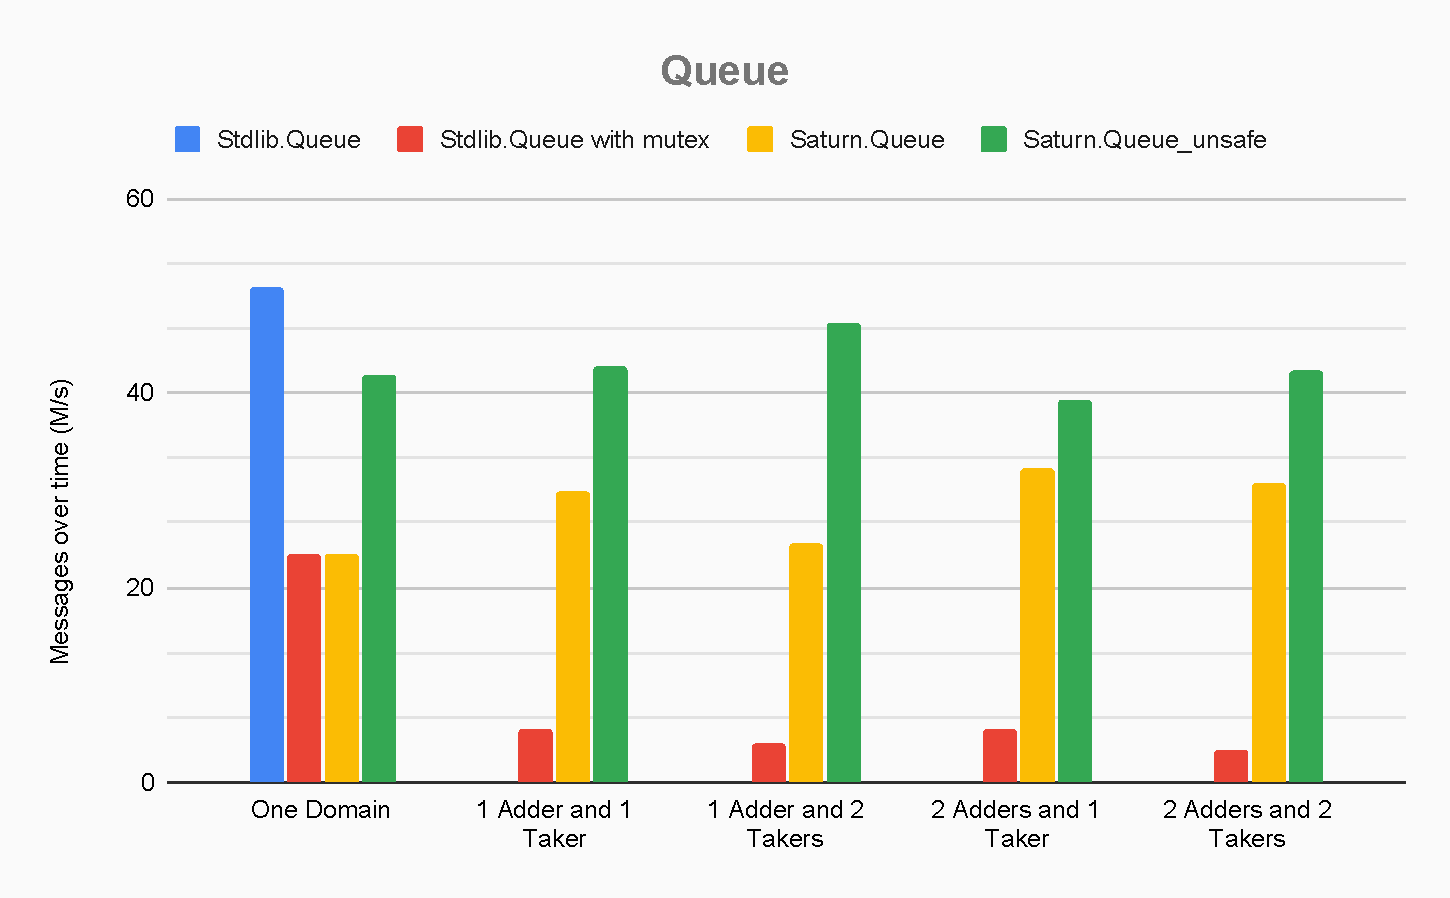
\includegraphics[width=0.55\linewidth]{images/Queue.pdf}
%     \onslide<2->{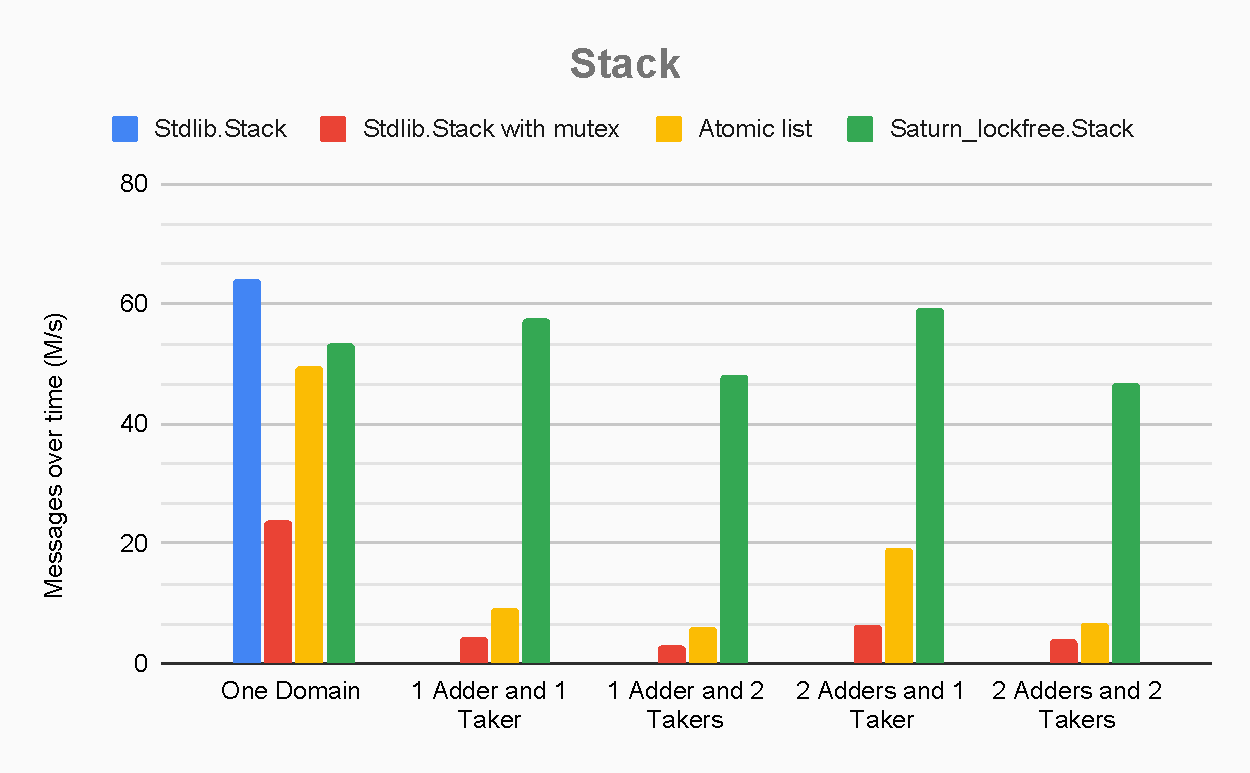
\includegraphics[width=0.55\linewidth]{images/Stack.pdf}}
%     \only<3>{\url{https://github.com/lyrm/saturn-benchmarks/}}
%  \end{frame}

  \begin{frame}{Is it any good ?}
    \centering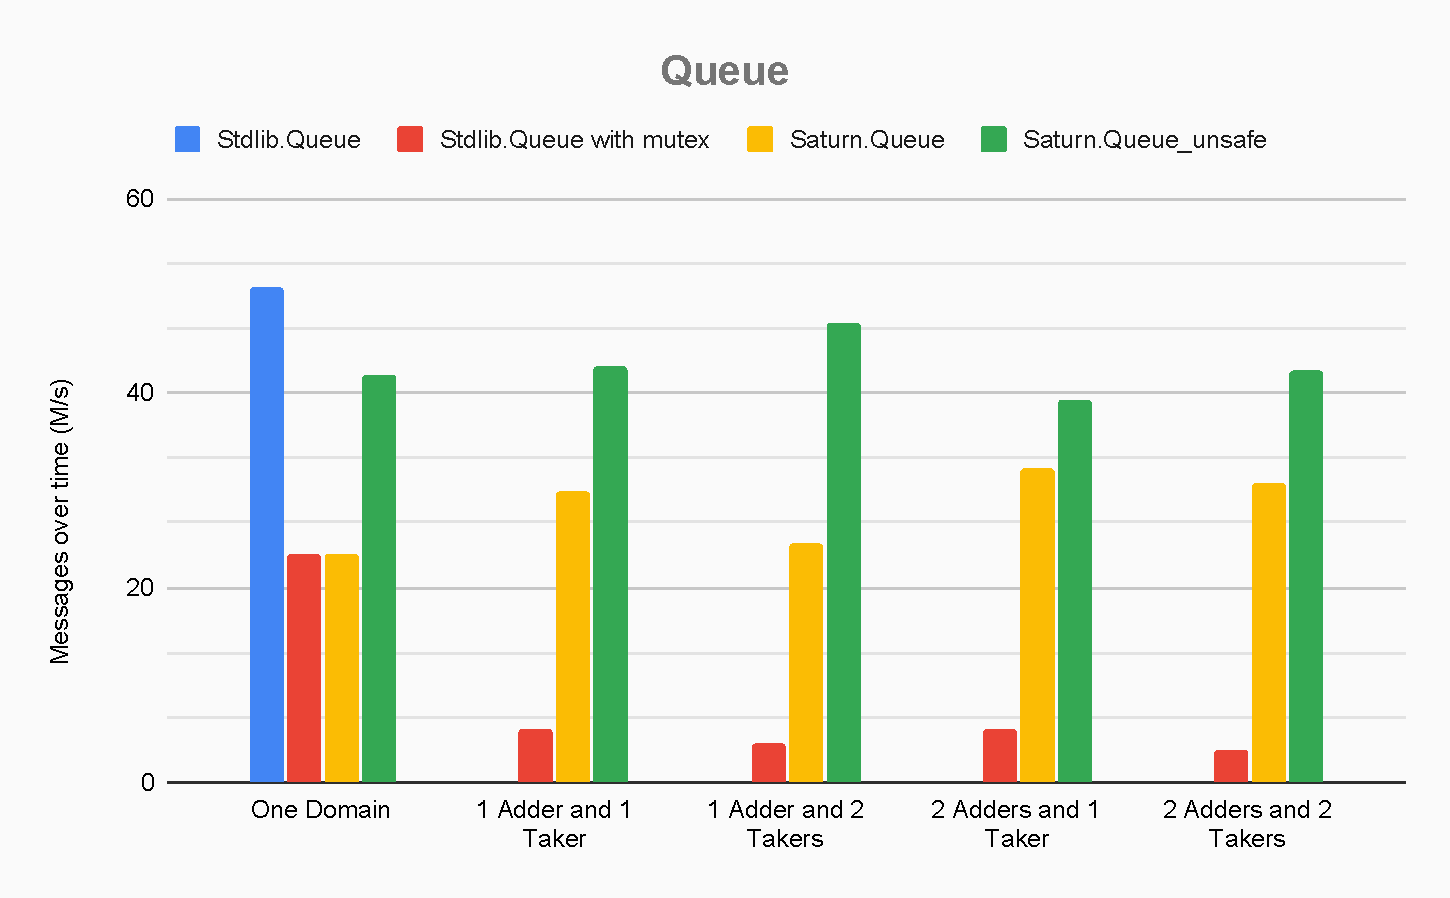
\includegraphics[width=0.8\linewidth]{images/Queue.pdf}
 \end{frame}


 \begin{frame}{Is it any good ?}
\centering
    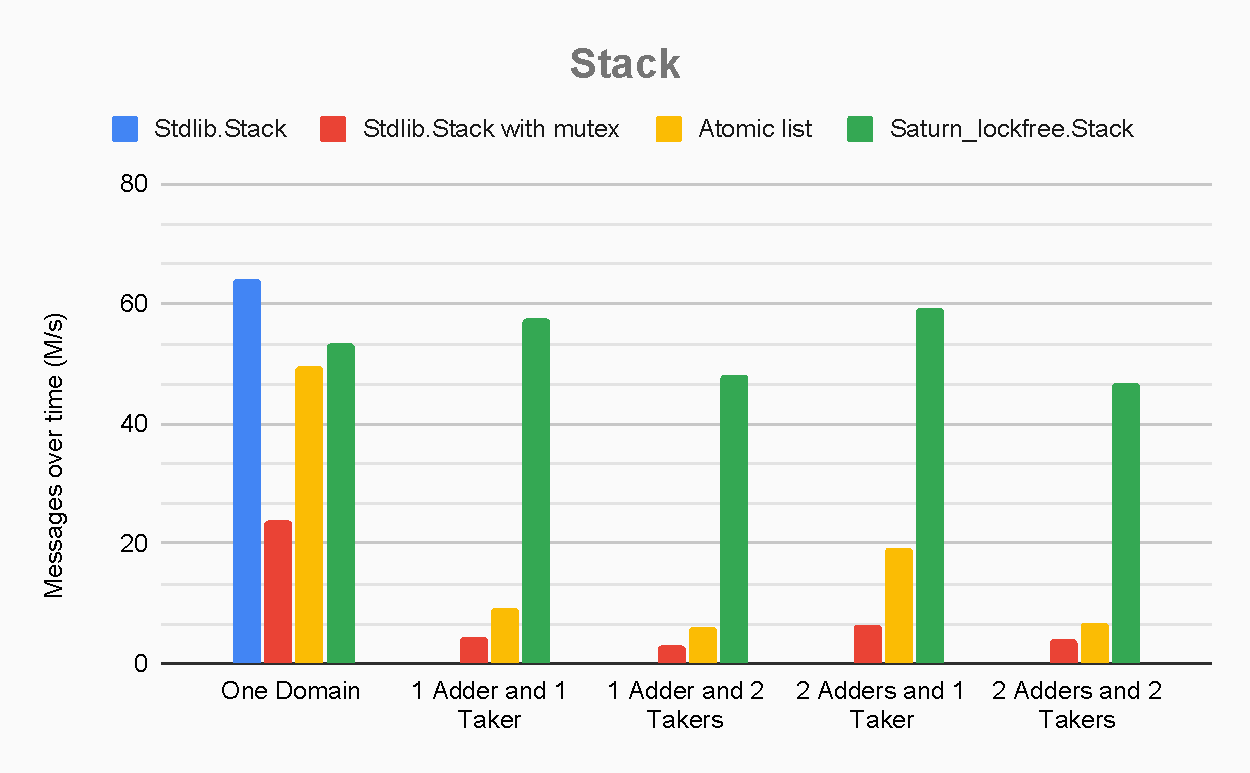
\includegraphics[width=0.8\linewidth]{images/Stack.pdf}
     \only<2>{\url{https://github.com/lyrm/saturn-benchmarks/}}
  \end{frame}


\begin{frame}{Formal verification}
\centering
\Large
\emph{Testing} a concurrent algorithm is hard due to the number of potential interleavings.
\vfill
\emph{Formal verification} is here to help us!
\vfill
\begin{tabular}{ccc}
        
\includegraphics[scale=0.7]{images/iris.png}
    &&
        
\includegraphics[scale=0.5]{images/coq.png}
\end{tabular}
\end{frame}

\begin{frame}[fragile]{From \OCaml to \Coq}
\centering
\small
\begin{minted}{ocaml}
let rec push t v =
  let old = Atomic.get t in
  let new_ = v :: old in
  if not (Atomic.compare_and_set t old new_) then (
    Domain.cpu_relax () ;
    push t v
  )
\end{minted}
\vspace{-6mm}
\hfill \OCaml
\medskip
\hrule
\hfill \Coq
\vspace{-6mm}
\begin{minted}{coq}
Definition stack_push : val :=
  rec: "stack_push" "t" "v" =>
    let: "old" := !"t" in
    let: "new" := ‘Cons( "v", "old" ) in
    ifnot: CAS "t" "old" "new" then (
      Yield ;;
      "stack_push" "t" "v"
    ).
\end{minted}
\end{frame}

\begin{frame}{Proving linearizability}
\centering
\Large
\begin{tabular}{ccccc}
    linearizability
  &&
    $\stackrel[\text{in SC}]{}{\simeq}$
  &&
    $\aspec{
      \mathrm{stack \mathhyphen inv}\ t
    }{
      \mathit{vs}
    }{
      \mathrm{stack \mathhyphen model}\ t\ \mathit{vs}
    }{
      \texttt{stack\_push}\ t\ v
    }{
      \mathrm{stack \mathhyphen model}\ t\ (v :: \mathit{vs})
    }{
      \texttt{()}
    }{
      \mathrm{True}
    }$
\end{tabular}
\vfill
\normalsize
\emph{Theorems for free from separation logic specifications} \\
Birkedal, Dinsdale-Young, Guéneau, Jaber, Svendsen \& Tzevelekos
\end{frame}

\begin{frame}{Relaxed memory model (future work)}
\centering
\large
\[
    \aspec{
      \mathrm{stack \mathhyphen inv}\ t
    }{
      v_0, \dots, v_n, \textcolor{red}{\mathcal{V}_0}, \dots, \textcolor{red}{\mathcal{V}_n}
    }{
      \mathrm{stack \mathhyphen model}\ t\ ((v_0, \textcolor{red}{\mathcal{V}_0}), \dots (v_n, \textcolor{red}{\mathcal{V}_n}))
    }{
      \texttt{stack\_push}\ t\ v, \textcolor{red}{\mathcal{V}}
    }{
      \mathrm{stack \mathhyphen model}\ t\ ((v, \textcolor{red}{\mathcal{V}}), (v_0, \textcolor{red}{\mathcal{V}_0}), \dots (v_n, \textcolor{red}{\mathcal{V}_n}))
    }{
      \texttt{()}
    }{
      \mathrm{True}
    }
\]
\vfill
\normalsize
\emph{Cosmo: a concurrent separation logic for multicore \OCaml} \\
Mével, Jourdan \& Pottier
\end{frame}

\begin{frame}[fragile]{Writing concurrent protocols in \Iris}
\small
\begin{minted}{coq}
Definition stack_inv t ι : iProp Σ :=
  ∃ l γ,
  ⌜t = #l⌝ ∗ meta l nroot γ ∗
  inv ι (
    ∃ vs, l ↦ lst_to_val vs ∗ stack_model₂ γ vs
  ).

Lemma stack_push_spec t ι v :
  <<< stack_inv t ι
  |   ∀∀ vs, stack_model t vs >>>
          stack_push t v @ ↑ι
  <<< stack_model t (v :: vs)
  |   RET (); True            >>>.
Proof.
  ...
Qed.
\end{minted}
\end{frame}

\begin{frame}[plain, noframenumbering]
\LARGE
\centering
Thank you for your attention!
\end{frame}

\end{document}
